\documentclass[xcolor=pdftex,dvipsnames,table]{beamer}
\usepackage{graphics}
\usepackage{amsmath,amssymb}
\usepackage{multicol}
\usetheme{Boadilla}
\usecolortheme[named=Red]{structure}
\setbeamercovered{transparent}
\setbeamertemplate{items}[circle]
\newcommand{\blue}[1]{{\color{blue} #1}}
\newcommand{\red}[1]{{\color{red} #1}}
\newcommand{\con}{\,|\,}

\newcommand*{\approxdist}{\mathrel{\vcenter{\offinterlineskip
\vskip-.25ex\hbox{\hskip.55ex$\cdot$}\vskip-.25ex\hbox{$\sim$}
\vskip-.5ex\hbox{\hskip.55ex$\cdot$}}}}
%%%%%%%%%%%%%%%%%%%%%%%%%%%%%%%%%%%%%%%%%%%%%%%%%%%%%%%%%%

\title[STAT585X Class project]{Changes in cultivated cropland soil in Iowa }
\author[Andreea L. Erciulescu]{Andreea L. Erciulescu}
\date{April, 2014}
\institute[ISU]{Iowa State University  \\ Statistics Department}


\begin{document}
%-------------------------------------title

\begin{frame}
\titlepage
\end{frame}
%--------------------------------------------------------------------

\begin{frame}
\frametitle{Outline}
\begin{itemize}
\item Motivation and problem description
\item Available data 
\item Data processing steps
\item Results
\item Conclusions and future work
\end{itemize}
\end{frame}

%---------------------------------------------------------------------------------

\begin{frame}
\frametitle{National Resources Inventory (NRI)}

\begin{itemize}
\item annual survey conducted collaboratively by USDA NRCS (Natural
Resources Conservation Services) and ISU Center for Survey Statistics and Methodology (CSSM)
\item to
provide status and trend estimates for natural resources on nonfederal lands in US
  \begin{itemize}
  \item Example of such estimates are soil erosion estimates in relation to land characteristics and programs.
  \end{itemize}
\end{itemize}
\end{frame}
%---------------------------------------------------------------------------------

\begin{frame}
\frametitle{Conservation Effects Assessment Project (CEAP)}

\begin{itemize}
\item series of surveys intended to quantify environmental
effects of conservation prctices and programs by hydrologic unit codes (HUCs)
\item CEAP sample is a subset of the NRI points classified as cultivated cropland
    \begin {itemize}
    \item Farmer interviews about on-farm practices  
  	\item Hydrologic, climate and soil databases
		\item APEX model
    \end{itemize}
\end{itemize}
\end{frame}


%------------------------------------------------------------------------------------------

\begin{frame}
\frametitle{United States territory divion into HUCs}
Local concerns regarding the existance of nitrates in drinking water, particularly in Des Moines

\begin{center}
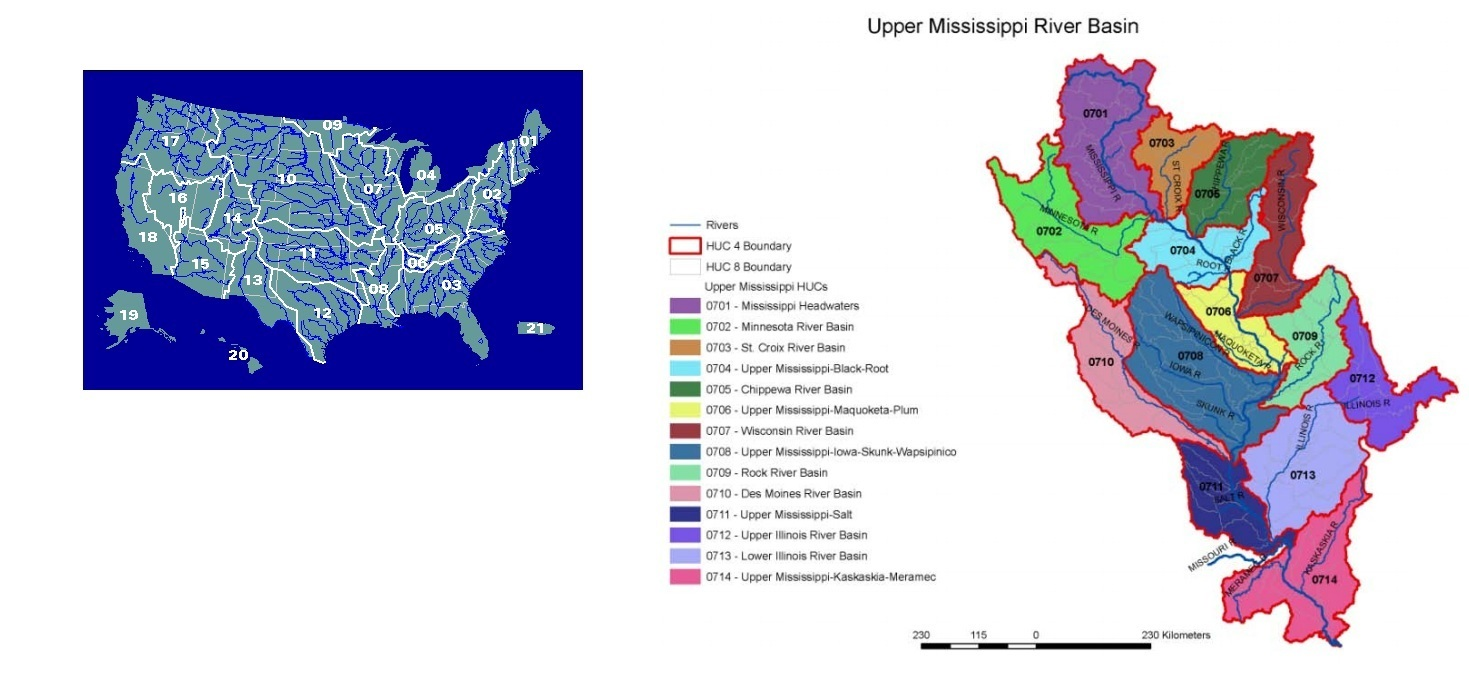
\includegraphics[width=10cm, height=5cm]{HUC2-4-8.jpg} 
\end{center}

\end{frame}

%------------------------------------------------------------------------------------------

\begin{frame}
\frametitle{Data - available}
 Crop Data Layer (CDL)\\


The CDL data is available at \href {CDL} {http://nassgeodata.gmu.edu/CropScape/} in the form of Tagged Image File (.tif) Format. We are interested in the state of Iowa data, available for the years of 2003-2007. The information consists of pixel counts and acreage values for different category of cropland data. Each of the category has an associated value (code), for example 1 stands for Corn and 5 stands for Soybean. A complete list of category codes, class names and colors for the USDA NASS CDL is available at \href{Codes}{http://www.nass.usda.gov/research/Cropland/docs/CDL_2013_crosswalk.htm}.

\end{frame}

%------------------------------------------------------------------------------------------

\begin{frame}
\frametitle{Data - available}

\begin{itemize}
\item Public Land Survey System (PLSS)\\

The PLSS data can be found on \href{PLSS}{http://http://www.geocommunicator.gov/GeoComm/lsis_home/home/index.htm} in the form of shapefiles. Information is available at both state and county levels.  
\item   GIS data on hydrologic basins\\

The GIS data can be found at \href{GIS}{ftp://ftp.igsb.uiowa.edu/gis_library/basins/} in the form of shapefiles. Information is available for the entire Des Moines River basin.

\item   Atlas of historical countyu boundaries (AtlasHCB)\\

The AtlasHCB data is available at \href{AtlasHCB}{http://publications.newberry.org/ahcbp/pages/Iowa.html} in the form of shapefiles. Information os available for the entire state of Iowa.

\item Census Topologically Integrated Geographic Encoding and Referencing database (Tigerweb) \\


The Census Tigerweb data is available at \href{Census}{http://tigerweb.geo.census.gov/tigerwebmain} for both national and regional leveles. Also, data for the hydrologic levels is available at 

\href{HydroCensus}{http://tigerweb.geo.census.gov/tigerwebmain/Files/tigerweb_tab10_hydro_poly_ia.html}. We are interested in the state of Iowa data, as well as the Des Moines River data. In particular, we are interested in the points coordinates. 

\end{itemize}


\end{frame}

%------------------------------------------------------------------------------------------

\begin{frame}
\frametitle{Data processing - CDL}


\begin{itemize}
\item download from \href {CDL} {http://nassgeodata.gmu.edu/CropScape/}, years 2003-2007
\item raster graphics images, spatial data
structures that divide the US teritory into pixels that store crop information. This type of data are
referred to as a ’grid,’ contrasted with ’vector’ data is used to represent points, lines, polygons. The
dimensions of files are very large
\item Raster package in R 
       \begin{itemize}
      \item uses sp package
      \item S4 method
       \item - the raster values from the files and to convert the cell numbers to coordinates and back
      \end{itemize}
\end{itemize}
\end{frame}
%------------------------------------------------------------------------------------------

\begin{frame}
\frametitle{2003 CDL data - Raster object attributes}
\begin{verbatim}
## class : RasterLayer
## dimensions : 11672, 17796, 207714912 (nrow, ncol, ncell)
## resolution : 30, 30 (x, y)
## extent : -52065, 481815, 1938165, 2288325 (xmin, xmax, ymin, ymax)
## coord. ref. : +proj=aea +lat_1=29.5 +lat_2=45.5 +lat_0=23 +lon_0=-96 +x_0=0 +y_0=0 +ellps=GRS80 +towgs84=0,0,0,0,0,0,0 ## data source : U:\classes\585X\data\cdl\CDL_2003_19.tif
## names : CDL_2003_19
## values : 0, 255 (min, max)

\end{verbatim}

\begin{itemize}
\item read the values for the region of interest using cell numbers and coordinates (xy) in the extraction method from the cellFromXY
\end{itemize}

\end{frame}
%------------------------------------------------------------------------------------------

\begin{frame}
\frametitle{Data processing - GIS, PLSS, AtlasHCB data}

\begin{itemize}
\item download and read in using maptool library in R
\item extract polygon information from the shapefiles
\item universal transverse
mercador (UTM) and we need to convert it to the longitude-latitude, then to the CRS with the
appropriate raster characteristics
\end{itemize}
\end{frame}

%------------------------------------------------------------------------------------------

\begin{frame}
\frametitle{Data processing - Tigerweb}

\begin{itemize}
\item pull Iowa data and Hydrologic data from web using the XML library in R
\item select the data on Des Moines River and 'create' the watershed region to get a significant number of points
\end{itemize}
%include maps
\end{frame}

%---------------------------------------------------------------------

\begin{frame}
\frametitle{Results}

\begin{table}[ht]
\tiny
\begin{center}
\caption{Proportions of crop by category, by year}
\begin{tabular}{cccccccccc}
  \hline
year  & corn & soybean & ... & ... & ... & .... & ... & ... & ... \\ 
  \hline
2003 & 0.0111 & 0.0609 & 0.0335 & 0.0220 & 0.0171 & 0.0254 & 0.0566 & 0.0840 & 0.0964 \\ 
2004 & 0.0292 & 0.0534 & 0.0442 & 0.0425 & 0.0568 & 0.0374 & 0.0442 & 0.0367 & 0.0448 \\ 
2005 & 0.0313 & 0.0659 & 0.0512 & 0.0494 & 0.0729 & 0.0411 & 0.0521 & 0.0449 & 0.0627 \\ 
2006 & 0.0292 & 0.0534 & 0.0442 & 0.0425 & 0.0568 & 0.0374 & 0.0442 & 0.0367 & 0.0448 \\ 
2007 & 0.0313 & 0.0659 & 0.0512 & 0.0494 & 0.0729 & 0.0411 & 0.0521 & 0.0449 & 0.0627 \\ 
\hline
\end{tabular}
\end{center}
\end{table}
\end{frame}

%---------------------------------------------------------------------%---------------------------------------------------------------------

\begin{frame}
\frametitle{Conclusions and future work}

Challenges
\begin{itemize}
\item big data 
\item coordinates in different measurement system
\item raster package uses sp package
\item different sources of data, need to choose useful, realible and (hopefully) not big data
\end{itemize}


Future work
\begin{itemize}
\item use the CDL data and the sampled CEAP points (data not publicly available) to compute crop estimates
\item shiny app ?
\end{itemize}

\end{frame}

%--------------------------------------------------------------
\begin{frame}
\frametitle{End}

\large{Thank you for your attention!}\\

\end{frame}
\end{document}